% -----------------------------------------------------------------------------
% UFRJ
% PPGI
% MAB 733 Sistemas Distribuídos
%
% Revisado em <não revisado>
% Autor: Cristiano Gurgel de Castro
% -----------------------------------------------------------------------------

\chapter{Desenvolvimento e Arquitetura}

Houve algumas tentativas de desenvolvimento da aplicação até conseguirmos a
comunicação com os diferentes tipos de serviços web. Iremos apresentar parte dos
problemas encontrados. Nas próximas seções são apresentadas as tentativas de
implementação do serviço até conseguirmos implementá-lo. São mostrados partes de
código, a arquitetura códigos e uma descrição de boa parte dos problemas
encontrados. 

\section{Tentativa de desenvolvimento no \NetBeansv}

O programa é composto por uma aplicação \desktop\ cliente Java de nome
\code{CalculatorGui}. Essa aplicação simples trata-se de uma calculadora que
efetua algumas operações básicas. 

Primeiramente foi desenvolvido um serviço web em Java para a implementação das 4
operações básicas. No projeto cliente, foi criada uma fachada para essa camada
de negócios: \code{IMathOperations} e duas implementações desta fachada:
\code{MathOperations}, que é local, e \code{RemoteMathOperations}. Esta última
utiliza contém os métodos para utilização de um \WebService. A arquitetura então
desenvolvida é representada na Fig.  \ref{fig:arquitetura:calc}. Um trecho do
código da classe \code{RemoteMathOperations} com a chamada ao método de soma do
serviço Web é mostrado no Código \ref{cod:add}.

\begin{figure}[htb]
  \centering
    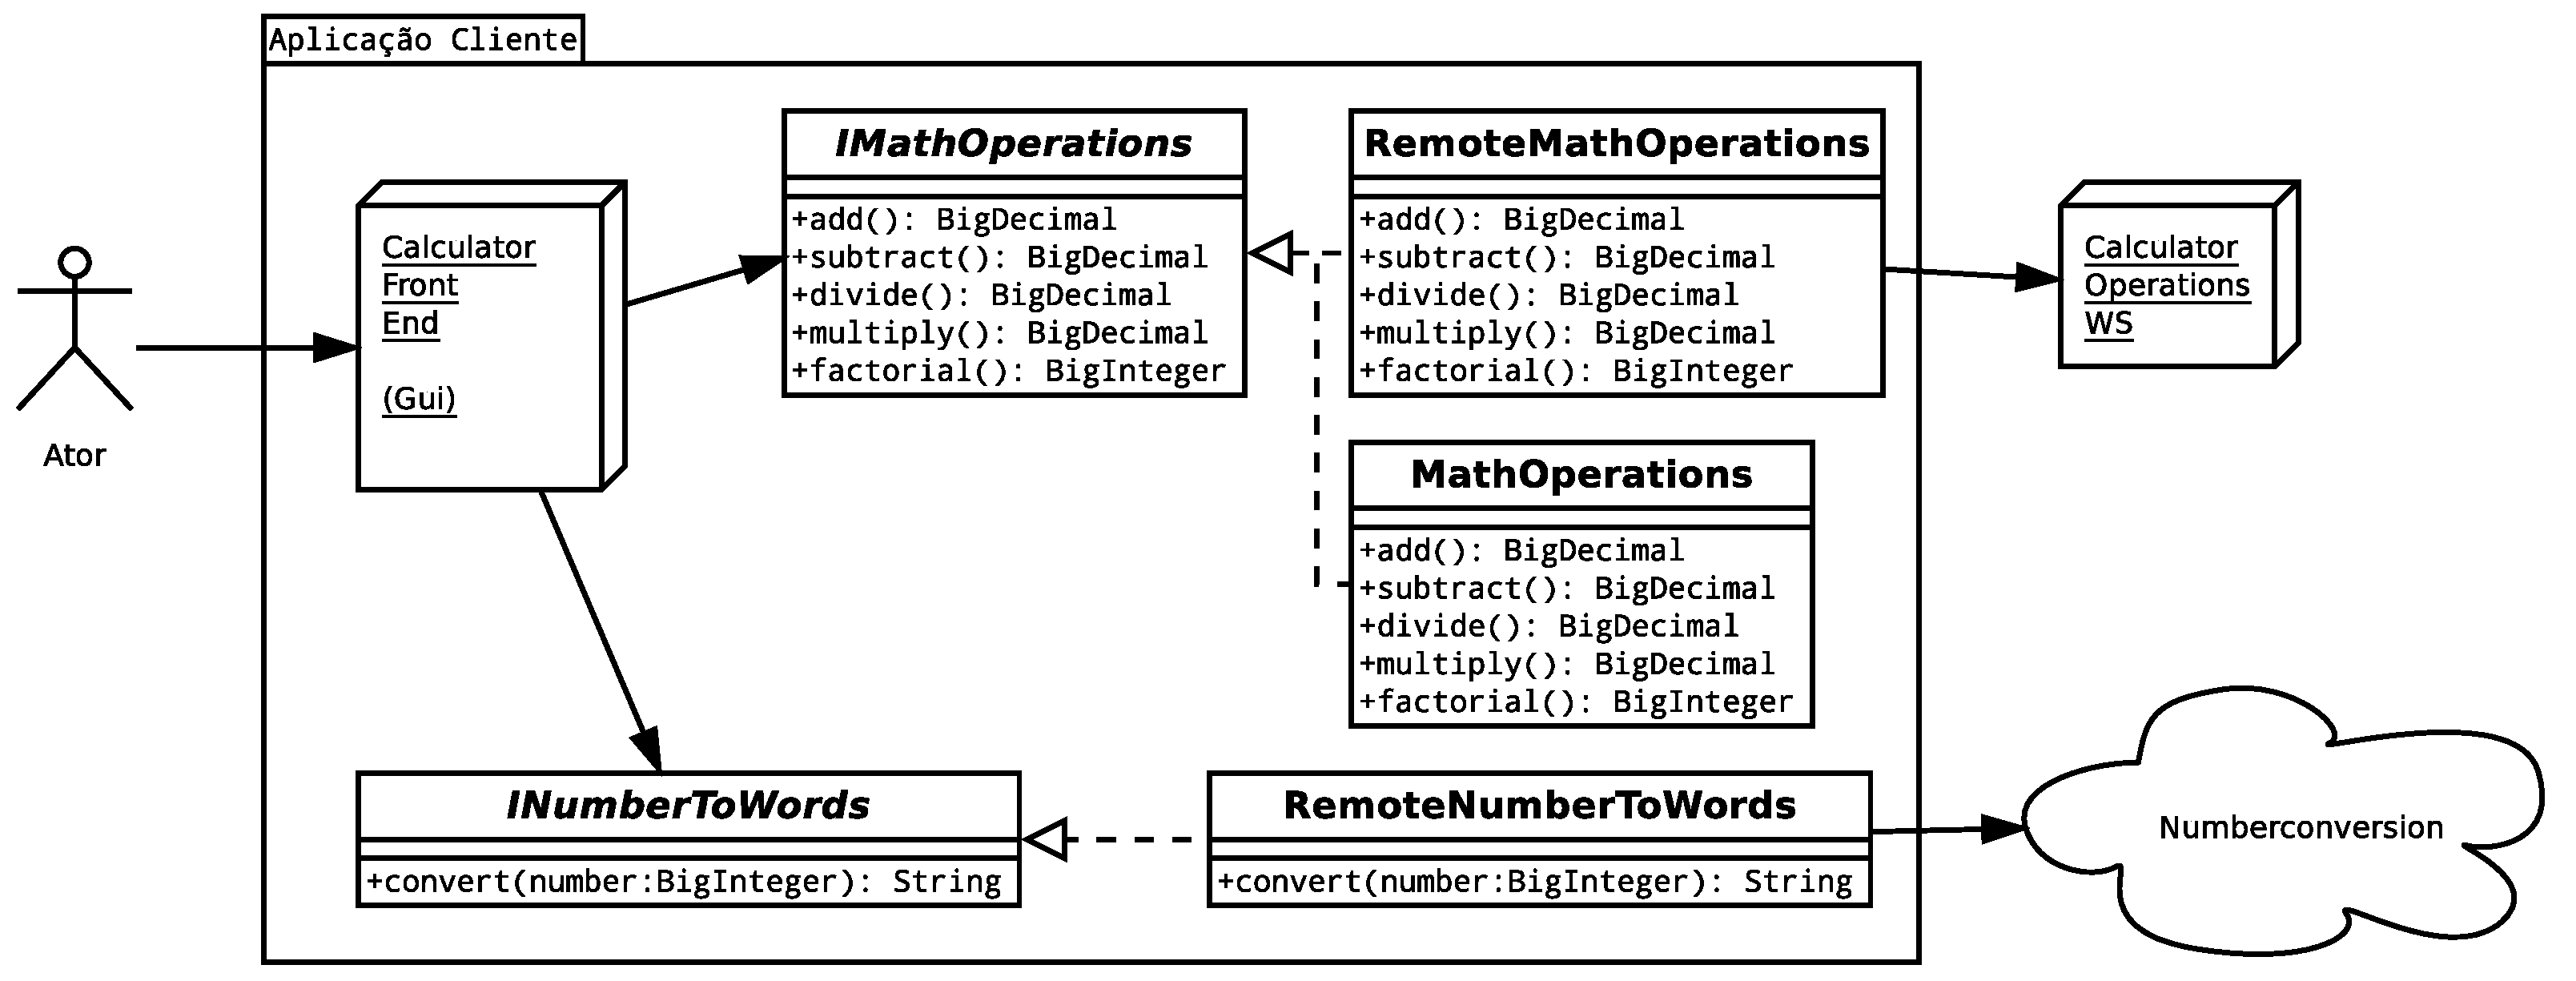
\includegraphics[width=\textwidth]{imgs/calculadora}
  \caption{Arquitetura da aplicação cliente.}
  \label{fig:arquitetura:calc}
\end{figure}

O serviço \code{CalculatorWebService} provê uma implementação das quatro
operações básicas. O \WebService\ foi criado
utilizando o IDE \NetBeansv\ juntamente com servidor de aplicação \Glassfish, o
qual já vem integrado à IDE e no qual foi hospedado o serviço. O \NetBeans\
provê uma funcionalidade muito prática de criação de \WebService s, através da
utilização da opção \textbf{Serviço Web} do Assistente de criação de projetos. O
\NetBeans\ automaticamente cria uma classe com a implementação do Serviço Web. O
usuário pode visualizar uma tela chamada \emph{Projeto} contendo uma
visualização amigável das operações efetuadas a serem implementadas no serviço
(ver Figura \ref{fig:arquitetura:design}). Através dessa tela, foram
configuradas as quatro operações que o \WebService\ deve fornecer: as quatro
operações básicas. Cada uma dessas operações recebem dois \code{float}s como
parâmetros e retornam um \code{float} como resultado.  Após a configuração das
operações, a tarefa seguinte foi inserir o código de implementação. Um trecho de
código exemplo, com a operação de adição do \WebService, é mostrado no código
\ref{cod:calculatorws}:

\begin{figure}[htb]
  \centering
  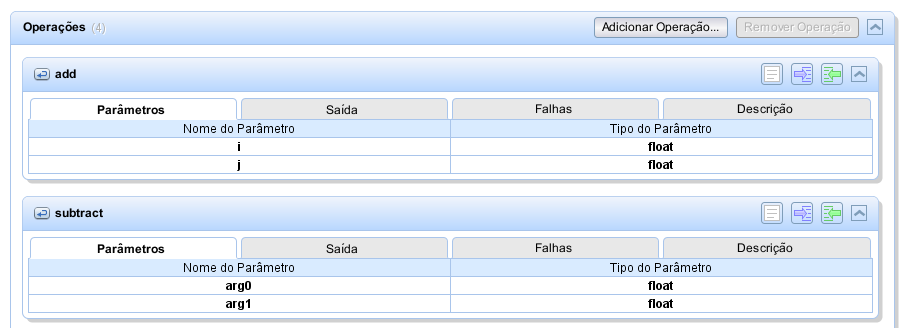
\includegraphics[width=\textwidth]{imgs/webservice-design}
  \caption{Tela de design de um \WebService}
  \label{fig:arquitetura:design}
\end{figure}

Dois serviços externos foram considerados: Um deles foi o \emph{Number
Converter} encontrado a partir do site \url{xmethods.net}. Segundo sua
descrição\footnote{Descrição encontrada em
\url{http://www.dataaccess.com/webservicesserver/numberconversion.wso}}
ele possui dois métodos: o primeiro (\code{NumberToWords}) contém um serviço de
escrita de número por extenso na língua inglesa, recebendo como parâmetro um
\code{inteiro}; o segundo (\code{NumberToDollars}) contém uma funcionalidade
semelhante para conversão para valores monetários em dólar. Para o presente
trabalho foi utilizado apenas o primeiro método: \code{NumberToWords}

Para o acesso ao serviço Web foi utilizada uma facilidade do \NetBeans\ na
aplicação cliente da calculadora: a criação de um ``Cliente para serviço Web''.
Esse componente da IDE foi adicionada ao projeto cliente de calculadora, e
através de um Assistente para a configuração. Um dos parâmetros informados foi a
URL do WSDL do serviço\footnote{a saber
\url{http://www.dataaccess.com/webservicesserver/numberconversion.wso?WSDL}}. Uma
funcionalidade \textbf{SAY} foi adicionada ao projeto para a chamada ao serviço. Uma
classe \code{NumberToWords} foi criada para a executar a chamada ao
\WebService. A chamada ao serviço web externo é mostrado no código
\ref{cod:numberconv}.

No entanto um erro de transporte mostrado no código \ref{cod:httperror}, foi
lançado durante a chamada de serviço. Interessante notar que um outro projeto
cliente Java foi criado para testar a comunicação com o serviço Web
\code{numberconversion} e a comunicação ocorreu sem maiores problemas. Para um
segundo teste de acesso ao serviço, Um outro cliente, dessa vez escrito na
linguagem \php\, também executou normalmente o acesso ao serviço. O Código
\ref{cod:phpclient} mostra o acesso ao serviço externo com um cliente \php. Para
contornar o problema, o código fonte do projeto Calculadora original, foi
exportado e importado no projeto cliente o qual conseguiu acesso ao \WebService\
e assim conseguimos executar a chamada.

Finalmente, passamos a implementação de um serviço em outra linguagem de
programação para utilização na calculadora. Testamos um serviço
\estrangeiro{Hello World} simples. Foi escolhida a linguagem de programação
\PHP\ para a criação de um outro serviço local, o código do aplicação
\estrangeiro{Hello World} é apresentado no Código \ref{cod:phphello}. No entanto
ao importar o cliente para utilização no cliente Java Utilizando o assistente do
\NetBeans\ nos deparamos com um problema que não conseguimos contornar: não se
conseguiu gerar o \estrangeiro{proxy} a partir do WSDL gerado a partir do \PHP
utilizando-se da biblioteca \code{NuSOAP} de classes. Primeiramente, o
assistente de criação de \proxy\ gerou uma mensagem de erro na criação do
WebService a partir do WSDL gerado pela biblioteca \code{NuSOAP} informando um
erro de impossibilidade de criação devido ao Estilo RPC. Foi tentado então
modificar o estilo do WSDL gerado de ``RPC'' para ``Document''. O \NetBeans\
conseguiu então gerar as classes \proxy\ para a utilização do serviço, porém ao
utilizar o serviço, deparamos com a seguinte mensagem de exceção: \code{Couldn't
create SOAP message due to exception: unexpected XML tag}.

Como não conseguimos a resolução, passamos a utilização do IDE \Eclipsev.

\section{Desenvolvimento no \Eclipsev}

Passamos a utilizar o \Eclipsev\ para tentar a comunicação com o serviço gerado
pelo código \PHP. Foram utilizados, integrado ao \Eclipse, o \ApacheTomcatv\ e o
\ApacheAxisDoisv. Primeiramente para os testes de aplicação, foi seguido o
tutorial de criação de um servidor e cliente através da utilização do
\ApacheAxisDoisv\footnote{\url{http://www.eclipse.org/webtools/community/tutorials/BottomUpAxis2WebService/bu_tutorial.html}}.
Primeiramente ao tentarmos criar um \textbf{Dynamic Web Project} tínhamos nos
deparado com o seguinte erro: \code{The Apache Axis2 Web service runtime in
Tomcat v7.0 Server does not support the service project ConverterProj.}. Ao
seguir o tutorial porém foi esclarecido que o erro era causado por não ter-se
habilitado o \estrangeiro{facet} \code{Axis2 Web Services} para o projeto o qual
gostaríamos de adicionar um serviço.

Então o próximo passo foi desenvolver um cliente de forma a consumir três
serviços: o serviço Java local gerado a partir do Tutorial apresentado no parágrafo
anterior (\code{Converter}), o serviço provido na web (\code{numberconversion})
e o serviço provido pelo servidor Apache também local escrito em \php. As
classes \estrangeiro{stub} para o acesso ao cliente foram criados através do
assistente \textbf{Web Service Client}. O código para utilizar os serviços Web a
partir dos \stub s gerados é mostrado no trecho de código
\ref{cod:javaeclipseclient}

Com a execução correta desse código partiu-se para a importação dos projetos
desenvolvidos anteriormente em \NetBeans\ para a plataforma \Eclipse. E assim
pudemos desenvolver a calculadora para utilizar também os serviços de um
\WebService\ local escrito em \PHP. A arquitetura final da aplicação é mostrada
na Fig. \ref{fig:arquitetura:final} 

\begin{figure}[htb]
  \centering
  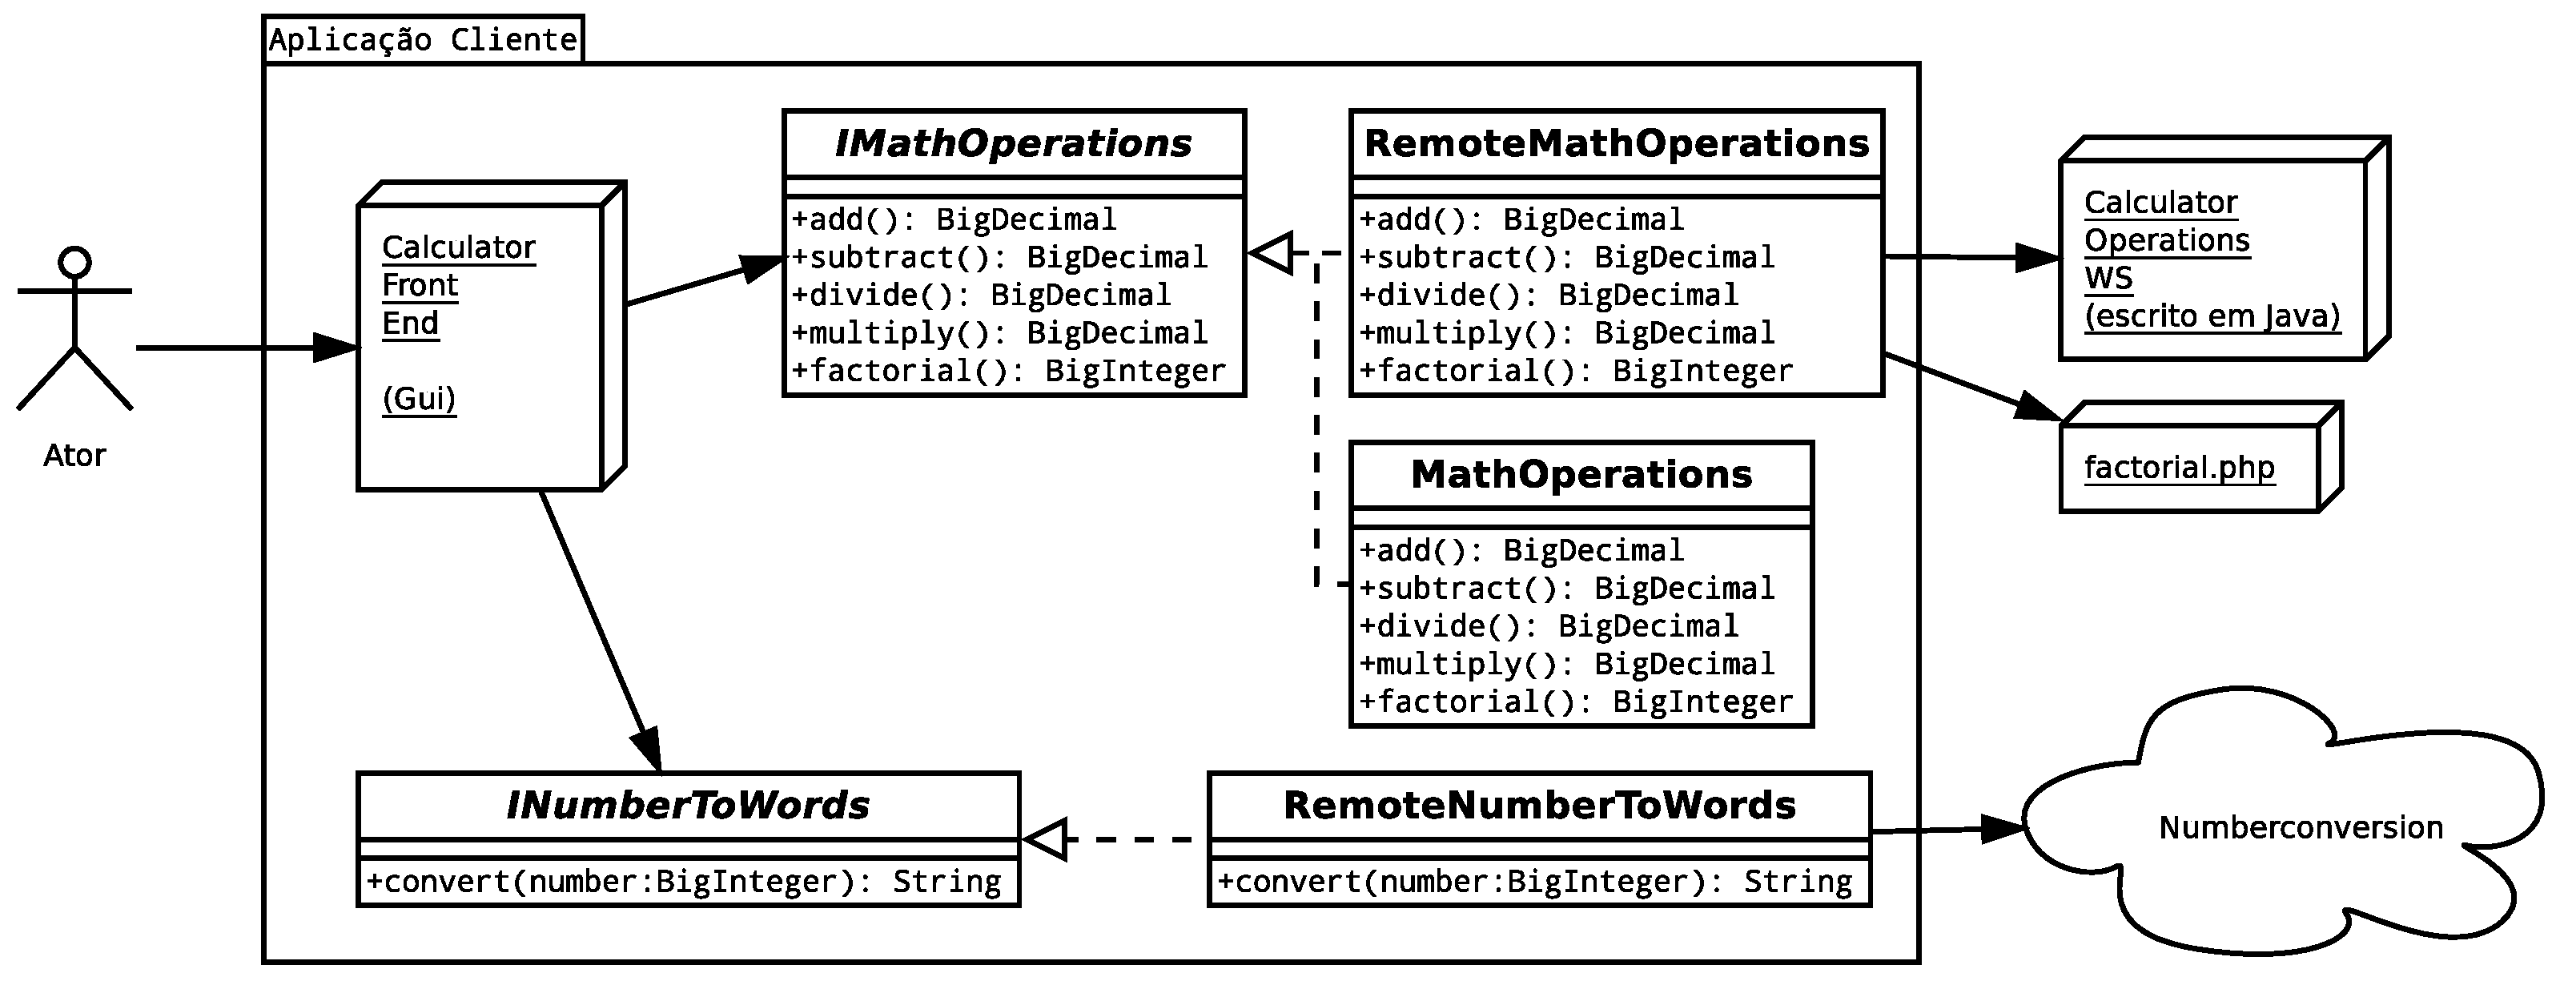
\includegraphics[width=\textwidth]{imgs/arquitetura_final}
  \caption{Arquitetura final da aplicação Calculadora escrita em Java}
  \label{fig:arquitetura:final}
\end{figure}

Um trecho de código do serviço PHP utilizado para a implantação do servidor de
cálculo do fatorial de um número é mostrado no Código \ref{cod:phpfactorial}. Os
trechos de código que requisitam os serviços web utilizados são mostrados nos
códigos \ref{cod:remote:math:eclipse} e \ref{cod:remote:conversion:eclipse}. 

